\documentclass[12pt]{article}


\usepackage[english]{babel}

% Set page size and margins
% Replace `letterpaper' with `a4paper' for UK/EU standard size
\usepackage[a4paper,top=2cm,bottom=2cm,left=3cm,right=3cm,marginparwidth=1.75cm]{geometry}

\usepackage[dvipsnames]{xcolor}
\definecolor{myblue}{RGB}{74, 144, 226}
\definecolor{myred}{RGB}{255, 2, 27}
%%%%%%%%%%%%%% Packages %%%%%%%%%%%%%%%%
\newtheorem{lemma}{Lemma}
%\usepackage{hyperref}
%\usepackage[...]{hyperref}
%\usepackage[colorlinks=true, allcolors=blue]{hyperref}
\usepackage[english]{babel}
\usepackage{amssymb}
\usepackage{underscore}
\usepackage{graphicx}
\usepackage{empheq}
\usepackage{booktabs}
\usepackage{tikz}
\newcommand*{\vertbar}{\rule[-1ex]{0.5pt}{2.5ex}}
\newcommand*{\horzbar}{\rule[.5ex]{2.5ex}{0.5pt}}
%% Some imports:
%\let\proof\relax
%\let\endproof\relax
%\let\example\relax
%\let\endexample\relax

%\usepackage{import}
\usepackage{float}
\usepackage{multirow}
\usepackage{amsmath}
% ,amsfonts,amssymb,amsthm
%\usepackage{subfigure}

\usepackage[ruled]{algorithm2e}
\usepackage{mathtools}
\usepackage[super]{nth}
\usepackage{caption}
\usepackage{subcaption}
\usepackage{graphicx}
%\usepackage{wrapfig}
\usepackage{verbatim} % comments
%\usepackage{comment}
%\renewenvironment{comment}{}{}
\usepackage{array}
\usepackage{supertabular}
\usepackage{longtable}
\usepackage{tabularx}
\usepackage{multirow}
\usepackage{colortbl}
\usepackage{fancyhdr}
%\usepackage{tcolorbox}
%\usepackage{tikz}
%\usetikzlibrary{math} %needed tikz library
%\usepackage[linesnumbered,ruled]{algorithm2e}
%\usepackage{pgf}
%\usepackage{pgfplots, pgfplotstable}
%\usetikzlibrary{fit,calc,positioning,decorations.pathreplacing,matrix}
%\usetikzlibrary{arrows}
%\usetikzlibrary{shapes}
%\usetikzlibrary{chains}
% Vector Styles
%\tikzstyle{load}   = [ultra thick,-latex]
%\tikzstyle{stress} = [-latex]
%\tikzstyle{dim}    = [latex-latex]
%\tikzstyle{axis}   = [-latex,black]
%\usepackage{pgffor}

%\usepackage{multido}
%\usepackage{calc}
%\usepackage{fp}
%\usepackage{xifthen}
%\usepackage{xargs}
\usepackage{etoolbox}
\DeclareMathAlphabet{\mathpzc}{OT1}{pzc}{m}{it}
\usepackage{breakcites} 
\usepackage[utf8]{inputenc}
\usepackage{helvet}
%\usepackage{geometry}
%\geometry{left=16mm, top=30mm, right=16mm, bottom=30mm}

%\usepackage{amssymb}
\usepackage{enumitem}
\usepackage{tabularx}
%\usepackage{xcolor}
\usepackage[absolute,overlay]{textpos}
%\usepackage{graphicx}
\usepackage{lipsum}
%\usepackage{caption}
\usepackage{multicol}
\usepackage{afterpage}
\usepackage{setspace}
\usepackage{parskip}
\usepackage{import} 
\usepackage[colorlinks=true,linkcolor=blue,allcolors=blue]{hyperref}%
\usepackage{hhline}
\graphicspath{{../figures/}}
%allcolors=blue

%%%%%%%%%%%%%% end Packages %%%%%%%%%%%%%%%%

%\pgfplotsset{compat=1.18}


\import{./}{Notations}

%\setlength{\parindent}{0cm}
%\noindent




\title{Rank Reduction Autoencoders - Enhancing interpolation on nonlinear manifolds.}
\author{Jad Mounayer$^{1,2,*}$, Sebastian Rodriguez$^{1,3}$, Chady Ghnatios$^{1,2}$, \\Charbel Farhat$^{4}$, Francisco Chinesta$^{1,5}$ \\ \\
$^1$PIMM, ENSAM Institute of Technology, 151 Boulevard de \\ l'Hôpital, 75013, Paris, France.\\
$^2$ PIMM Lab, SKF
Research Chair, Arts et Metiers
Institute of \\ Technology, Paris,
France\\
$^3$ESI Group Chair, PIMM, ENSAM Institute of Technology, \\ 151 Boulevard de l'Hôpital, 75013, Paris, France. \\
$^4$ Stanford University, Department of Aeronautics and Astronautics \\ Department of Mechanical Engineering and Industrial for \\ Computational and  Mathematical Engineering, \\ 496 Lomita Mall, Stanford, 94305, CA, USA. \\
$^5$RTE
Research Chair, PIMM, ENSAM Institute of Technology, \\ 151 Boulevard de l'Hôpital, 75013, Paris, France.\\
}



\begin{document}


\maketitle

\begin{abstract}
Is it possible to reproduce the solution of a physical problem in a parametric space if we only know the solution for a few parameters? In other words, can we interpolate between available solutions to find new ones? This problem was the main reason behind the development of many methodologies (e.g. PODi, optimal transport). Yet, the effectiveness of most currently available techniques is reduced significantly when the problem has many features (i.e. high-rank solution matrices, with many large singular values). In general, High-rank matrices are hard to deal with. For instance, the efficiency of most reduction techniques (e.g. POD, PGD, PCA), or any other low-rank methods decreases when the number of dominant singular values increases. But, is it possible to reduce the dimension of high-rank matrices by finding an approximation of a lower rank? 

Linearly, the truncated SVD is our best alternative. However, its reduction capabilities are limited, since we almost need all the features to represent the matrix when many singular values are large. Accordingly, research is directed to find low-rank approximations using nonlinear functions, specifically, Autoencoders with reduced latent spaces. However, a smaller latent space makes it difficult, even impossible in practice, to reconstruct the original matrix. Therefore, some architectures were proposed to expand the data dimensionality in the latent space while enforcing the resulting matrix to have a low rank (e.g. IRMAE, LoRAE). Their results show that Autoencoders with longer, but low-rank, latent spaces lead to better Autoencoders, specifically for interpolation. In this paper, we present Rank Reduction Autoencoders (RRAE), designed to strongly enforce a low rank on long latent spaces by finding the basis that represents it. We present two formulations, strong/weak ones to achieve what's proposed.
Further, we propose two ways (linear/nonlinear ones) to interpolate between the curves in the latent space. We show that both formulations can interpolate between curves with one/two-dimensional parametric spaces even when a linear interpolation is used. Finally, we showcase the effectiveness of RRAEs by using them to interpolate between physical solutions generated by the Avrami crystallization model. We show that RRAEs preceded by a POD can filter noisy data, their interpolating abilities are not reduced if a wrong dimension of the parametric space is chosen, and both the linear/nonlinear interpolation techniques proposed can lead to effective nonlinear interpolation.

\begin{comment}
Reducing the computational overhead of multiple methods depends on the fraction of the relevant features (i.e. the number of dominant singular values). Problems with many large singular values, known as high-rank, are very hard to deal with. Not only does the efficiency of multiple reduction techniques (e.g. POD, PGD, PCA) drop significantly, but every low-rank technique found in the literature becomes of little use. In this article, we present a way to transform any high-rank matrix (or a problem with many important features) into a lower-rank one by using Rank Reduction Autoencoders (RRAE). RRAEs are used to find a latent space that is representable with only a few dominant singular values. In this article, we demonstrate that by using nonlinearities, reduction to only one significant singular value is often possible. We propose two techniques for constructing latent spaces with highly reduced dimensionality, typically of dimension 1,  a Weak and a Strong formulation. The two formulations are then tested for an interpolation task on three equation-generated problems, as well as on a set of real-world data. We show that by using a logically chosen model architecture, both methodologies are robust and fairly easy to train. They both have errors that are less than $2\%$ over all the presented examples for both test and train sets, and their latent spaces indeed have only one dominant singular value. We finally sum up with future research that includes testing RRAEs on problems with multiple parameters, and for other applications in the latent space.

\end{comment}

\end{abstract}


\textit{Keywords}: Rank Reduction Autoencoder, Non-linear interpolation, Low-rank latent space, Non-linear model-order reduction, Singular Value Decomposition, Dominant singular values, High-rank matrices.



\section{Introduction}\label{sec:intro}
Numerical methods, such as the Finite Element Method (FEM) \cite{zienkiewicz2005finite}, or the Finite Difference Method \cite{smith1985numerical} are popular due to their ability to reproduce real physical systems. However, an increase in the complexity of the system directly affects the computational overhead, hence the speed, of these methods. Thus, multiple modalities, such as Model Order Reduction (MOR) techniques, have been presented in the literature to circumvent this problem.

Amongst the most popular MOR techniques are the Proper Orthogonal Decomposition (POD) \cite{rowley2004model, kerschen2005method}, the Proper Generalized Decomposition (PGD) \cite{ladeveze1985famille,rodriguez2019non, chinesta2014pgd}, and the Principal Component Analysis (PCA) \cite{labrin2020principal, gonzalez2018kpca}. The efficiency of these techniques made them lay the basic principles of many others, specifically those that tackled interpolation between different solutions. For instance, the POD with interpolation (PODI) \cite{tezzele2019shape, nguyen2022efficient, rama2020towards}, or the sparse PGD (sPGD) \cite{chinesta2011short, sancarlos2023regularized}, were developed to create high dimensional parametric surrogates, with the ability to reproduce the solution in an entire parametric space with only a few samples. 

The methods presented above, as well as every low-rank technique (e.g. \cite{srebro2003weighted, liu2012robust, udell2016generalized, davenport2016overview}), all depend on the ability to represent the space by a finite set of features, which is usually of much smaller dimension than the original feature set. Mathematically speaking, if multiple solutions are stacked into a matrix,  only a few singular values of the matrix are dominant compared to the others (i.e. a low-rank matrix). When this assumption is not valid, the presented techniques would provide little to no improvement at all, meaning that the dimensionality of the original problem may not be reduced efficiently. The aforementioned methods, and many other reduction techniques, lose most of their efficiency when dealing with high-rank matrices, making it challenging to create efficient surrogates for the correct prediction of physical phenomena.

On the other hand, machine learning algorithms are being used in almost every field due to their speed and their ability to approximate nonlinear behavior. Countless model architectures include Multiple Layer Perceptrons \cite{popescu2009multilayer, seiffert2001multiple, mitra1995fuzzy, tang2015extreme}, Recurrent Neural Networks \cite{medsker2001recurrent, salehinejad2017recent, medsker1999recurrent}, and Convolutional Neural Networks \cite{albawi2017understanding, gu2018recent, li2021survey}. 

The nonlinearity in Neural Networks encouraged researchers to use them for interpolation \cite{berrada2020training, rigol2001artificial}. One of the techniques that showed a great ability to interpolate is Autoencoders. The idea of an autoencoder is to learn two functions. First, an encoding function moves the data into what we call the latent space, which is usually of a different dimension than the original space. This is followed by the decoding function that brings us back to the original values. Autoencoders have been introduced in the 1990s for dimensionality reduction and feature learning \cite{hinton1993autoencoders}. Their ability to learn generative models of data made them a compelling match with machine learning algorithms. Accordingly, autoencoders with Neural Networks as their encoding/decoding functions have been successfully used in many applications such as speech recognition \cite{vachhani2017deep, feng2014speech}, medical applications \cite{deng2019towards, shin2012stacked}, robotics \cite{park2018multimodal, sergeant2015multimodal}, and others \cite{bank2023autoencoders}. In practice, models enforce some characteristics of the latent space to avoid learning the identity function. For instance, larger latent spaces could be used to find Koopman embeddings \cite{lusch2018deep}. On the other hand, a better understanding of the data can be established when the latent space is smaller \cite{wang2016auto}. Even though Autoencoders appeared to be very promising, their efficiency is limited, especially for data reduction/interpolation (Section \ref{sec:insights}), since it is usually very hard to reconstruct the original data from a small dimension in the latent space. Accordingly, multiple enhancements, such as Sparse, Denoising, and Variational autoencoders \textcolor{red}{Citations}, have been proposed to alleviate these issues. Specifically, the Implicit Rank-Minimizing Autoencoder (IRMAE) \cite{jing2020implicit}, and the Low-Rank Autoencoder (LoRAE) \cite{mazumder2023learning} showcased how increasing the latent space dimension while enforcing a low-rank achieves better results, including interpolation.

In the following article, we present Rank Reduction Autoencoders (RRAE), which consist of autoencoders that find a reduced basis of the latent space that can be later used for interpolation. This is achieved by the use of two architectures: strong/weak formulations. Furthermore, we propose two ways (linear/nonlinear) to perform interpolation in the latent space. Since the reduced basis is supposed to represent the entire latent space, interpolating between curves becomes more efficient. 

The present paper is structured as follows: section \ref{sec:HT} presents the architecture and both formulations proposed. Next, we explain our interpolation strategy in section \ref{sec:interp}. Afterward, we demonstrate, based on a simple example, why an enlarged latent space with a low rank is more efficient than a smaller latent space (regular autoencoders) in section \ref{sec:insights}. Then, both formulations are tested on a variety of curves in section \ref{sec:Nuemrical}. Subsection \ref{sec:numerical_example} covers one-parameter examples where we show that RRAEs with both formulations have better interpolation abilities than the regular Autoencoder on challenging examples. The generalization to more parameters is discussed and tested in section \ref{sec:generalisation}, where we show that by finding a reduced basis of the latent space, a bilinear interpolation is sufficient! RRAEs are then tested on physical data in subsection \ref{sec:physical}, where we test their abilities to filter noise and learn interpolation when a wrong dimension of the parametric space is given. Finally, we conclude and discuss the future aspects and the limitations of the proposed model in section \ref{sec:conclusions}. Our results show that RRAEs with both formulations, and both interpolation techniques, can interpolate on nonlinear manifolds, even when the solution matrix is high-rank.


\section{Rank Reduction Autoencoders (RRAEs)}\label{sec:HT}
The idea of Rank Reduction Autoencoders (RRAEs) is to find a reduced basis that can represent the latent space. To be consistent, we start by defining autoencoder notations.

Let $\{X_i\}_{i\in [1, D]} \in \mathbb{R}^T$ be a set of $D$ series of observations, each of length $T$. We define our input $X\in \mathbb{R}^{T\times D}$ with $X_i$ as its $i$th column. Let, $Y \in \mathbb{R}^{L\times D}$ with $L$, the chosen dimension of the latent space. We also define the encoding map $e: \mathbb{R}^{T\times D} \xrightarrow{} \mathbb{R}^{L\times D}$ and the decoding map $d: \mathbb{R}^{L\times D} \xrightarrow{} \mathbb{R}^{T\times D}$. The Vanilla autoencoder can be written as the following two operations,
\begin{equation}
        Y = e(X), \qquad \tilde{X} = d(Y).
\end{equation}
In practice, we usually demand that the output of the autoencoder gives us back the original data, hence the loss usually reads,
\begin{equation}
    \mathcal{L}(X, \tilde{X}) = \Vert X-\Tilde{X}\Vert_2, \quad \text{where,} \quad \Vert \cdot\Vert_2 \text{ is the L2-norm}.
\end{equation}
The idea behind RRAEs is to enforce the latent matrix to have a low rank. In other words, let $Y = U^y\Sigma^yV^y$ be the Singular Value Decomposition (SVD) \cite{stewart1993early, nakatsukasa2017accuracy} of Y, and let $\{\sigma^y_i\}_{i \in [1, r]}$ be the sorted diagonal values of $\Sigma^y$, $r$ being the rank of Y. We want the following,
\begin{equation}
    \sigma^y_k \gg \sigma^y_j, \qquad \forall j \in [k+1, r], \qquad k \ll r.
\end{equation}
Another way to define the requirement is by the truncated SVD,
\begin{equation}\label{eqn:trunc}
    Y = \sum_{i=1}^r\sigma^y_iU^y_i(V^y)_i^T \qquad\Rightarrow\qquad Y\approx \sum_{i=1}^k\sigma^y_iU^y_i(V^y)_i^T,
\end{equation}
where $U^y_i$ is the $i$th column of $U^y$ and $(V^y)_i^T$ is the $i$th row of $V^y$. In other words, we can write $Y_d$, the $d$th column of $Y$ as,
\begin{equation}\label{eqn:alphas}
    Y_d = \sum_{j=1}^k\alpha^d_jW_j, \qquad \text{with }\alpha^d_j\in\mathbb{R}, \quad W_j\in\mathbb{R}^L, \quad \forall d \in [1, D].
\end{equation}
In other words, for a specified number of nodes $k$, each column of $Y$ is defined by $k$ constants and $k$ vectors. In other words, the vectors $W_j$ form a basis for the latent space. By stacking all the vectors $W_j$ as columns of a matrix $W$, we write \eqref{eqn:alphas} in matrix form as follows,
\begin{equation}\label{eqn:mat_form}
    Y =( A\cdot W^T)^T, \qquad \text{with: } A_{i,j}=\alpha_j^i, \quad A \in \mathbb{R}^{D\times k}, \quad W \in \mathbb{R}^{L\times k},
\end{equation}
with $(\cdot)$ denoting the dot product. Based on \eqref{eqn:alphas}, and \eqref{eqn:mat_form}, we propose two formulations to enforce the latent space to have a reduced basis. The architecture is sketched in figure \ref{fig:mdoel_arch}. 
\tikzset{every picture/.style={line width=0.75pt}} %set default line width to 0.75pt  
\begin{figure}

       

\tikzset{every picture/.style={line width=0.75pt}} %set default line width to 0.75pt        

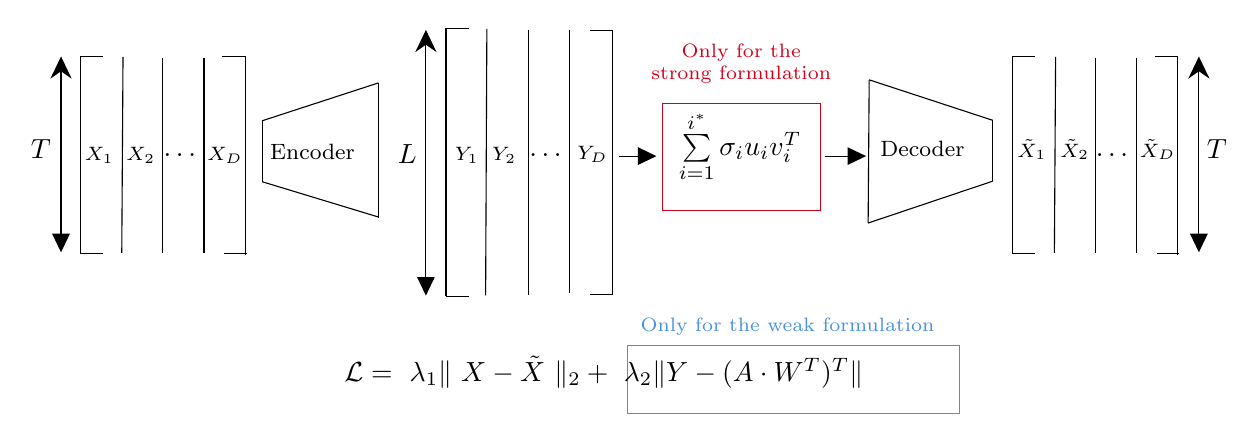
\begin{tikzpicture}[x=0.75pt,y=0.75pt,yscale=-1,xscale=1]
%uncomment if require: \path (0,329); %set diagram left start at 0, and has height of 329

%Straight Lines [id:da21499615368111846] 
\draw    (37,108.56) -- (37,203.67) ;
%Straight Lines [id:da16326946357296768] 
\draw    (37,108.56) -- (47.89,108.56) ;
%Straight Lines [id:da16265931324232152] 
\draw    (37,203.67) -- (47.89,203.67) ;
%Straight Lines [id:da5083389594267504] 
\draw    (116.56,204.33) -- (116.56,108.67) ;
%Straight Lines [id:da3615318503641125] 
\draw    (117.22,203.7) -- (106.33,203.7) ;
%Straight Lines [id:da9354769223516279] 
\draw    (116.22,108.6) -- (105.33,108.6) ;
%Straight Lines [id:da9284204806788381] 
\draw    (57.67,108.87) -- (57.07,203.27) ;
%Straight Lines [id:da9687380676381745] 
\draw    (76.67,109.25) -- (76.67,203.25) ;
%Straight Lines [id:da30039595434321] 
\draw    (96.67,109.25) -- (96.67,203.25) ;
%Straight Lines [id:da782396384119824] 
\draw    (124.67,139.67) -- (180.67,121.42) ;
%Straight Lines [id:da9238744798761502] 
\draw    (124.67,169) -- (180.67,186) ;
%Straight Lines [id:da44599235940336523] 
\draw    (180.67,121.42) -- (180.67,186.33) ;
%Straight Lines [id:da6964885949042201] 
\draw    (213.3,95.06) -- (213.3,224.17) ;
%Straight Lines [id:da06959562543054565] 
\draw    (213.3,95.06) -- (224.19,95.06) ;
%Straight Lines [id:da030633764479459424] 
\draw    (213.3,224.17) -- (224.19,224.17) ;
%Straight Lines [id:da3263511981591738] 
\draw    (293.52,223.5) -- (293.52,96.17) ;
%Straight Lines [id:da40502884422960217] 
\draw    (293.52,223.5) -- (282.63,223.5) ;
%Straight Lines [id:da8961788198500589] 
\draw    (293.52,96.3) -- (282.63,96.3) ;
%Straight Lines [id:da9774520960600939] 
\draw    (232.97,95.37) -- (232.37,223.77) ;
%Straight Lines [id:da5075505519042733] 
\draw    (252.97,95.75) -- (252.97,223.75) ;
%Straight Lines [id:da21045855349115494] 
\draw    (272.97,95.75) -- (272.97,222.75) ;
%Straight Lines [id:da754710144489299] 
\draw    (124.67,139.67) -- (124.67,169) ;
%Straight Lines [id:da7099185888654047] 
\draw    (417.17,119.92) -- (476.67,139.42) ;
%Straight Lines [id:da66143724081499] 
\draw    (476.67,168.75) -- (416.67,188.92) ;
%Straight Lines [id:da31064466545771574] 
\draw    (417.17,119.92) -- (416.67,188.92) ;
%Straight Lines [id:da5393972903258972] 
\draw    (476.67,139.42) -- (476.67,168.75) ;
%Straight Lines [id:da022156106633165695] 
\draw    (296.67,156.67) -- (311.67,156.67) ;
\draw [shift={(314.67,156.67)}, rotate = 180] [fill={rgb, 255:red, 0; green, 0; blue, 0 }  ][line width=0.08]  [draw opacity=0] (8.93,-4.29) -- (0,0) -- (8.93,4.29) -- cycle    ;
%Straight Lines [id:da38115442380124565] 
\draw    (395.67,156.67) -- (410.67,156.67) ;
\draw [shift={(415.67,156.67)}, rotate = 180] [fill={rgb, 255:red, 0; green, 0; blue, 0 }  ][line width=0.08]  [draw opacity=0] (8.93,-4.29) -- (0,0) -- (8.93,4.29) -- cycle    ;
%Shape: Rectangle [id:dp7709069667907207] 
\draw  [color={rgb, 255:red, 208; green, 2; blue, 27 }  ,draw opacity=1 ] (317.4,131.47) -- (393.67,131.47) -- (393.67,182.67) -- (317.4,182.67) -- cycle ;
%Shape: Rectangle [id:dp24666081940562967] 
\draw  [color={rgb, 255:red, 74; green, 144; blue, 226 }  ,draw opacity=1 ] (300.6,248) -- (460.89,248) -- (460.89,280.67) -- (300.6,280.67) -- cycle ;
%Straight Lines [id:da9073615867889311] 
\draw    (27.8,111.67) -- (27.8,200) ;
\draw [shift={(27.8,203)}, rotate = 270] [fill={rgb, 255:red, 0; green, 0; blue, 0 }  ][line width=0.08]  [draw opacity=0] (8.93,-4.29) -- (0,0) -- (8.93,4.29) -- cycle    ;
\draw [shift={(27.8,108.67)}, rotate = 90] [fill={rgb, 255:red, 0; green, 0; blue, 0 }  ][line width=0.08]  [draw opacity=0] (10.72,-5.15) -- (0,0) -- (10.72,5.15) -- (7.12,0) -- cycle    ;
%Straight Lines [id:da1988310735559562] 
\draw    (203.6,98.87) -- (203.6,220.87) ;
\draw [shift={(203.6,223.87)}, rotate = 270] [fill={rgb, 255:red, 0; green, 0; blue, 0 }  ][line width=0.08]  [draw opacity=0] (8.93,-4.29) -- (0,0) -- (8.93,4.29) -- cycle    ;
\draw [shift={(203.6,95.87)}, rotate = 90] [fill={rgb, 255:red, 0; green, 0; blue, 0 }  ][line width=0.08]  [draw opacity=0] (10.72,-5.15) -- (0,0) -- (10.72,5.15) -- (7.12,0) -- cycle    ;
%Straight Lines [id:da7075949415859115] 
\draw    (486.33,108.56) -- (486.33,203.67) ;
%Straight Lines [id:da776447423867771] 
\draw    (486.33,108.56) -- (497.22,108.56) ;
%Straight Lines [id:da40114415684531135] 
\draw    (486.33,203.67) -- (497.22,203.67) ;
%Straight Lines [id:da24114735322590564] 
\draw    (565.89,204.33) -- (565.89,108.67) ;
%Straight Lines [id:da8606039915940866] 
\draw    (566.56,203.7) -- (555.67,203.7) ;
%Straight Lines [id:da6175875067439736] 
\draw    (565.56,108.6) -- (554.67,108.6) ;
%Straight Lines [id:da9114789567469446] 
\draw    (507,108.87) -- (506.4,203.27) ;
%Straight Lines [id:da9606142652454763] 
\draw    (526,109.25) -- (526,203.25) ;
%Straight Lines [id:da3463806230867499] 
\draw    (546,109.25) -- (546,203.25) ;
%Straight Lines [id:da3635085614733373] 
\draw    (576.02,111.67) -- (576.02,200) ;
\draw [shift={(576.02,203)}, rotate = 270] [fill={rgb, 255:red, 0; green, 0; blue, 0 }  ][line width=0.08]  [draw opacity=0] (8.93,-4.29) -- (0,0) -- (8.93,4.29) -- cycle    ;
\draw [shift={(576.02,108.67)}, rotate = 90] [fill={rgb, 255:red, 0; green, 0; blue, 0 }  ][line width=0.08]  [draw opacity=0] (10.72,-5.15) -- (0,0) -- (10.72,5.15) -- (7.12,0) -- cycle    ;

% Text Node
\draw (38,151.2) node [anchor=north west][inner sep=0.75pt]  [font=\scriptsize]  {$X_{1}$};
% Text Node
\draw (58,151.2) node [anchor=north west][inner sep=0.75pt]  [font=\scriptsize]  {$X_{2}$};
% Text Node
\draw (97,151.2) node [anchor=north west][inner sep=0.75pt]  [font=\scriptsize]  {$X_{D}$};
% Text Node
\draw (127.33,149.67) node [anchor=north west][inner sep=0.75pt]  [font=\footnotesize] [align=left] {Encoder};
% Text Node
\draw (216.3,151.23) node [anchor=north west][inner sep=0.75pt]  [font=\scriptsize]  {$Y_{1}$};
% Text Node
\draw (234.3,151.23) node [anchor=north west][inner sep=0.75pt]  [font=\scriptsize]  {$Y_{2}$};
% Text Node
\draw (275.3,150.73) node [anchor=north west][inner sep=0.75pt]  [font=\scriptsize]  {$Y_{D}$};
% Text Node
\draw (421.33,148.17) node [anchor=north west][inner sep=0.75pt]  [font=\footnotesize] [align=left] {Decoder};
% Text Node
\draw (308,101.2) node [anchor=north west][inner sep=0.75pt]  [font=\scriptsize,color={rgb, 255:red, 208; green, 2; blue, 27 }  ,opacity=1 ] [align=left] {\begin{minipage}[lt]{69.37pt}\setlength\topsep{0pt}
\begin{center}
Only for the \\strong formulation
\end{center}

\end{minipage}};
% Text Node
\draw (305.8,233.2) node [anchor=north west][inner sep=0.75pt]  [font=\scriptsize,color={rgb, 255:red, 74; green, 144; blue, 226 }  ,opacity=1 ] [align=left] {Only for the weak formulation};
% Text Node
\draw (12,147.6) node [anchor=north west][inner sep=0.75pt]    {$T$};
% Text Node
\draw (188.8,149.8) node [anchor=north west][inner sep=0.75pt]    {$L$};
% Text Node
\draw (324.2,134) node [anchor=north west][inner sep=0.75pt]    {$\sum \limits_{i=1}^{i^{*}} \sigma _{i} u_{i} v_{i}^{T}$};
% Text Node
\draw (163.07,251.73) node [anchor=north west][inner sep=0.75pt]    {$\mathcal{L} =\ \lambda _{1} \| \ X-\tilde{X} \ \Vert _{2} +\ \lambda _{2} \| Y-(A\cdot W^T)^T\Vert $};
% Text Node
\draw (76,154.07) node [anchor=north west][inner sep=0.75pt]    {$\dotsc $};
% Text Node
\draw (252.13,154.07) node [anchor=north west][inner sep=0.75pt]    {$\dotsc $};
% Text Node
\draw (487.33,147.2) node [anchor=north west][inner sep=0.75pt]  [font=\scriptsize]  {$\tilde{X}_{1}$};
% Text Node
\draw (525.13,154.07) node [anchor=north west][inner sep=0.75pt]    {$\dotsc $};
% Text Node
\draw (508,147.2) node [anchor=north west][inner sep=0.75pt]  [font=\scriptsize]  {$\tilde{X}_{2}$};
% Text Node
\draw (546.33,147.2) node [anchor=north west][inner sep=0.75pt]  [font=\scriptsize]  {$\tilde{X}_{D}$};
% Text Node
\draw (578.56,147.6) node [anchor=north west][inner sep=0.75pt]    {$T$};


\end{tikzpicture}

\caption{Schematic showing the autoencoder in use as well as both methodologies. There are two terms in the loss function for the \textcolor{myblue}{Weak formulation}. On the other hand, there's an additional step before the decoder for the \textcolor{myred}{Strong formulation}.}
\label{fig:mdoel_arch}
\end{figure}
\newpage
\begin{enumerate}
    \item \underline{The Weak formulation:} This formulation is based on \eqref{eqn:mat_form}. After choosing the number of nodes $k$, we generate two trainable matrices of sizes $A \in \mathbb{R}^{D\times k}$, and $W \in \mathbb{R}^{L\times k}$. Afterward, we reduce the number of dominant singular values of the latent space by adding a term to the loss as seen in blue in figure \ref{fig:mdoel_arch}. By doing so, we are implicitly asking the Neural Network to find the values of constants $\alpha^d_j$ and vectors $W_j$ in \eqref{eqn:alphas}, and hence imposing the latent space to be represented by the reduced basis of the chosen size (i.e. low-rank latent space). We can say that the method finds PGD-like vectors that span the space, since we ask the Neural Network to find a basis, without enforcing the orthogonality of the vectors. Accordingly, the formulation gains some of the benefits and limitations of a PGD. On the one hand, we are finding a basis, so generalization over the test should be better since the basis should span the space of the parameters already seen in training. On the other hand, a larger number of modes could be required to represent the entire solution. 
    
    We will refer to this method as the Weak formulation since at the end of the training, the second term of the loss could still be large, meaning we might need more modes ($k^*>k$) to represent the latent space $Y$ correctly.

    \underline{Note for training:} Since in \eqref{eqn:alphas}, the constants $\alpha$ can be anything, but the vectors $W_j$ are normalized, we normalize each column of matrix $W$ after every gradient descent. In addition, our initial guess of $A$ and $W$ is normalized, so we use a bigger learning rate for those matrices compared to the rest of the Neural Network. The main reason is to allow the Neural Network to change significantly the values of the coefficients $\alpha_j^d$ even if the rest of the Neural Network doesn't need/can't sustain larger learning rates (more details in Section \textcolor{red}{AAA}).
    
    \item \underline{The Strong formulation:} Unlike the weak formulation, this architecture enforces, in a strong manner, the dimension of the reduced basis of the latent space. Similarly to the first formulation, we choose the number of modes $k$. Then, as seen in red in figure \ref{fig:mdoel_arch}, a truncated SVD (up to the $k$th singular value) of the latent space is given to the decoder, instead of the latent space itself. Accordingly, the input of the decoder will have exactly $k$ dominant singular values. In contrast to weak formulation, we can say that the strong formulation computes a POD-like basis since the vectors are by construction orthogonal. The orthogonality of the basis vectors, as well as limiting the loss function to one term should both make training and interpolating easier. On the other hand, backpropagation through the singular value decomposition is not common in practice, so it could lead to unexpected behavior in some frameworks where it is not implemented correctly.
\end{enumerate}
In both formulations, the main idea is to find a reduced basis of the latent space and enforce that the basis has a low dimension $k$. In the remainder of the paper, we show that both formulations lead to much better interpolation between curves with one/two parameters. We also show how RRAEs can reduce noise and computational overhead when combined with a POD, and they can perform training even if $k$ isn't chosen to be the original dimension of the parametric space. 

\section{Interpolation in the latent space}\label{sec:interp}
Since both formulations previously proposed find a reduced basis of a small dimension for the latent space, we propose two ways to perform interpolation in the latent space. Our work in this paper will be limited to interpolation but future research will include other tasks such as data generation and downstream classification tasks.

What motivated us to propose this application is the limitations of linear interpolation between solutions when the solution matrix is high-rank. Take, for instance, sinusoidal curves shifted by a scalar $p$ (i.e. $\sin(x+p)$). As can be seen in figure \ref{fig:sin}, interpolating linearly between the curves corresponding to parameters $p_0 = 0$ and $p_1 = \pi$ to find the middle curve at $p^*= \pi/2$ (i.e. simply the sum divided by two) leads to the horizontal line at zero, instead of finding the correct curve shifted towards the middle.
\begin{figure}[!b]
    \centering
    \includegraphics[clip, trim=0.4cm 0cm 0cm 1cm, width=1.1\textwidth]{sin.pdf}
    \caption{Figure showing the result when interpolating linearly between two shifted sin curves, showing why linear interpolation is not a good idea for problems with multiple dominant singular values.}
    \label{fig:sin}
\end{figure}
By sending the data into a longer latent space with a low rank, we believe we will be able to find a space where we can interpolate linearly before sending the data back to the original space with the decoder. 

Both proposed formulations allow us to approximate the latent space by \eqref{eqn:alphas} or \eqref{eqn:mat_form}. Now say, every series of observations $X_i$ is tied to a vector of parameters $\mathbf{p}_i \in \mathbb{R}^P$. Accordingly, and since each column $W_j$ is the same for every column of Y, we can only interpolate between the coefficients $\alpha_j^d$, as we can say,
\begin{equation}
    Y_d = \sum_{j=1}^k\alpha^d_jW_j, \qquad \Longrightarrow \qquad Y(\textbf{p}_i) = \sum_{j=1}^k\gamma_j(\textbf{p}_i)w,
\end{equation}
where each $\gamma_j: \mathbb{R^P} \xrightarrow{} \mathbb{R}$, could be any mapping, that maps all the training parameters to the corresponding $\alpha_j^d$, and allows us to interpolate when used on new values of the parameter $p$. 

\underline{Note:} In other words, we interpolate between the coefficients in matrix $A$!

Throughout the paper, we show that for every example presented a linear/bilinear interpolation is enough. For instance, for a parameter space of dimension one, and each $j$, we can sort the values of $\alpha_j^d$ based on their corresponding parameter values $p_i$ and write,
\begin{equation}
    \gamma_j(\mathbf{p}^*) = \gamma_j(p^*) = \alpha_m + \frac{\alpha_{m+1}-\alpha_{m}}{p_{m+1}-p_{m}}(p^*-p_{m}).
\end{equation}
where we distinguish between the \textbf{bold} notation for vectors and non-bold for scalars, $m$ is the index of the largest value of $p$ that is smaller than $p^*$, and both $p_0 = \alpha_0 =0$ for the equation to be valid for any $i\in[1, d]$.

Similarly, bilinear interpolation is performed between the four closest values of $\alpha_j^d$ from the top right, top left, bottom right, and bottom left respectively (for details, refer to Appendix \textcolor{red}{AAA}).

Finally, for higher dimensional cases, more elaborated techniques could be used for interpolation (e.g. the sPGD), or even a Neural Network. Yet, the drawback of using a Neural Network is that we would need a Neural Network for every mapping $\gamma_j$. In other words, as many Neural Networks as modes! Even though we show an example later in the paper where a Neural Network works very well, interpolating linearly between the coefficients (as shown in multiple examples in what follows) would work well in practice since the RRAE already did the linearisation job. 

\section{Insights behind RRAEs}\label{sec:insights}
Autoencoders were originally introduced with smaller latent dimensions for feature recognition and data reduction. Overall, Vanilla autoencoders try to find only a few features that represent the data before giving these back to the decoder. The papers that presented the IRMAE \cite{jing2020implicit}, and LoRAE \cite{mazumder2023learning} provided many examples showing that longer low-rank latent spaces lead to better results in interpolation, data generation, and downstream classification. In this section, we explain by two examples why and when longer low-rank latent spaces can overcome Vanilla autoencoders. The idea is to show why and when a long latent space of rank $k$ leads to better results than simply a latent space of dimension $k$.

\underline{1- Longer latent spaces lead to more flexibility in encoding:} As has been shown in many applications (e.g. Koopman Theory), a larger dimension leads to more linear behavior. Accordingly, by enlarging the latent space and asking the Neural Network to only use a reduced version of the matrix (i.e. both our Weak and Strong formulations), we allow the encoder to find more linear embeddings in the latent space, to then choose a few of them. Accordingly, for the same training parameters, while a regular autoencoder might find highly nonlinear coefficients to fit the training data, RRAEs find more ``linear" coefficients. Even though both could lead to great results on the training data, when interpolating (especially linearly in the latent space), the Vanilla autoencoder wouldn't have the right interpolations over the test set. Note that we don't claim to have done the impossible. Any Neural Network can overfit the data without learning the actual dynamics. 

As we show later in this section for curves parameterized with one parameter, Vanilla Autoencoders can be as efficient as RRAEs if the curves are highly nonlinear but easily separable. However, as can be seen in Section \ref{sec:Nuemrical}, RRAEs can interpolate between harder one-parameter curves and other two-parameter ones where the Vanilla AE fails. This is expected since both our Weak and Strong formulations have the advantage of building a basis in the latent space instead of finding random parameters. Once we have more than one parameter (i.e. more than one basis vector in the latent space), the strong formulation is finding an orthogonal basis (similar to a POD), while the weak formulation is finding a non-orthogonal one (similar to a PGD). Accordingly, if the test data have the same dynamics as the training ones, they should be representable by the basis already created in the latent space. The Vanilla Autoencoder on the other hand finds any values that help the decoder retrieve the solution. Accordingly, interpolating linearly, especially with multiple parameters, can lead to terrible interpolation results.

\underline{2- Longer latent spaces are easier to decode:} A long latent matrix of rank $k$ includes exactly as much information as a matrix of length $k$ with full rank. In other words, the decoder does not receive any more information when longer, but low-rank latent spaces are used. However, decoding with much longer latent spaces is easier since duplicated data is given to the network. For instance when $k=1$, a Vanilla autoencoder's latent space will contain only a constant per solution (say $c_i$). However, a longer latent space would include linear combinations as $\alpha_lc_i$ where $l \in [1, L]$. So the bigger the latent space, the more duplicated data is given to the decoder which can help it in untangling the relationships between parameters. Since the amount of data given is the same, we believe that a powerful decoder (e.g. many layers) should be able to reconstruct the data in a regular autoencoder anyway. In other words, smaller decoders can be used with RRAEs, and in complicated examples (e.g. pictures with multiple parameters, or curves that intersect multiple times), this could lead to better results over the training data. 

To explain further the arguments presented above, we test Vanilla Autoencoders and both our formulations on two examples characterized by one parameter. The first example we propose is shifted $\sin$ curves, since curves have a simple nonlinearity they are hard to separate (nonmonotonic and cross each other multiple times). The second example we propose is stair-like curves. In this example, we create highly nonlinear curves (different supports, different numbers of jumps, etc.) that are easier to separate (since they are monotonic and rarely cross each other). The equations used to define the columns of our input matrix $X$ in each case are,
\begin{equation}
\begin{cases}
    X_d(t_v,\, p_d) = f_{shift}(t_v, \, p_d) = \sin(t_v-p_d\pi), \hspace{0.1cm}\qquad\quad p_d \in [0, 1.5], \quad t_v \in \mathbb{R}^T, \\[1.2ex]
    X_d(t_v, \,p_d) = f_{stair}(t_v,\, p_d, \, \text{args}) 
\end{cases}
\end{equation}
where $t_v \in \mathbb{R}^T$ is a vector of time at which observations are done, and $f_{stair}$ is defined by the following algorithm,\\[2ex]
\begin{algorithm}[H]
\SetKwInput{Input}{Input}
\SetKwInput{Output}{Output}

\Input{$\mathbf{p} \in \mathbb{R}^P$, $t_v \in \mathbb{R}^T, (\text{Ph}_0, \text{Amp}_0,\kappa, y_0, w) \in \mathbb{R}$}

\For{$p \text{ in } \mathbf{p}$}{
    ~\\
    $\text{Amp} = p$\\[1.6ex]
    $\displaystyle\text{Ph} = \text{Ph}_0+\kappa(\text{Amp}-\text{Amp}_0)$\\[1.6ex]
    $g(t) = \text{Amp}\sqrt{t}\sin(w(t-\text{Ph}))-y_0$\\[1.6ex]
    $\displaystyle h(t) = \left(\frac{\left|g(t)\right|+g(t)}{2}\right)^5$\\[1.6ex]
    $f_p(t_v)=\text{cumsum}(g(t_v))$
}
\Output{$f_p(t_v)$ for every parameter $p$.}
\caption{Algorithm to find $f_{stair}$ for a list of parameters $\textbf{p}$.}
\end{algorithm}
In this paper, we choose the initial parameters of the stair function to be,
\begin{equation}
    \begin{cases}
        \text{Ph}_0 = 0.875, \qquad \text{Amp}_0=1\\
        \kappa = 2.286, \qquad y_0 = 2.3, \qquad w = 2\pi.
    \end{cases}
\end{equation}
Training is performed over 14 values of $p_d$ that are equidistant. We then test on 20 values randomly chosen inside the training domain. The large number of tests is to guarantee that the models are learning the dynamics and not just the training curves and some tests nearby. Since the curves depend on one parameter, we use a Vanilla Autoencoder with a scalar latent space, and an RRAE with a latent space of length 240 and rank one for both the weak and strong formulations, we fix every other training parameter for the comparison to be fair. The details of the hyperparameters and architecture choices can be found in Appendix \textcolor{red}{AAA}. The relative error over all $p$ values for both the train and test sets is documented in the following table,
\begin{table}[!h]
    \centering
    \begin{tabular}{|c|c|c|}
        \hline
        & Error on Train (in \%) & Error on Test (in \%) \\
        \hline
        Vanilla AE & 2.46 & 31.26\\
        \hline
        RRAE (Strong) & 1.35 & 2.4\\
        \hline
        RRAE (Weak) & 3.71 & 7.3\\
         \hline
\end{tabular}
\caption{Table showing the relative error (in \%) for all three architectures on both the train and test set for shifted sin curves.}
\label{fig:table_shift_sin}
\end{table}

It can be seen from the high relative error of the Vanialla Autoencoder that it is overfitting the data, even though the same training hyperparameters are used for all three architectures. In addition, and as will be seen in multiple examples in the paper later on, the strong formulation has the lowest error on the train set. This shows that even if an encoder/decoder of the same size was used for the RRAE and a Vanilla AE,  it is easier for the decoder in the RRAE to find better results because of the numerous duplicates in the latent space. To further understand the significance of the results, we depict the predictions of all three architectures in figure \ref{fig:sin_shift_test}.
\begin{figure}[!t]
    \centering
    \includegraphics[clip, scale=0.38, trim=2.6cm 1cm 0cm 0cm]{sin_shift_plot_test.pdf}
    \caption{Figure showing the predictions of Vanilla Autoencoders and RRAEs with both formulations of four particular values of $p$ in the test set.}
    \label{fig:sin_shift_test}
\end{figure}
We chose on purpose two values of $p$ next to the boundaries of the parametric domain (i.e. $p=0.06$ and $p=1.31$), as well as two other values randomly picked. As can be seen in the figure, The Vanilla Autoencoder's predictions (in blue) are close to the true curves (in grey) for some values of $p$ (to the left), but are completely different for other $p$-values to the right. On the other hand, the Strong formulation's predictions (in green), fit closely the curves for all the values of $p$. The weak formulation though is doing as well as the strong formulation over all the values of $p$ except for the smallest one where it is as bad as the regular Autoencoder. According to the claims we established before, it is expected that the RRAE can find more ``linear'' coefficients that facilitate interpolation, but is this what's happening here?

To validate our hypothesis, we draw the interpolated coefficients in figure \ref{fig:sin_shift_latent}. It is important to note that the coefficients are defined differently between the RRAE and the Vanilla AE. On the one hand, we remind the reader that the latent space for RRAEs can be written as in \eqref{eqn:mat_form}. However, since we only use one mode in this example, $A \in \mathbb{R}^D$ is simply a vector of coefficients (one for each curve, between which we interpolate). Figure \ref{fig:sin_shift_latent} shows the values inside vector $A$ plotted against the corresponding parameter for every curve for both the weak and strong formulations. On the other hand, since the latent space of the Vanilla autoencoder is of length one, its latent space is only a constant per curve (again, between which we interpolate) and hence we draw the latent space against the corresponding parameters for the Vanilla AE.
\begin{figure}
    \centering
    \includegraphics[clip, scale=0.38, trim=3.6cm 1cm 0cm 0cm]{sin_shift_plot_latent.pdf}
    \caption{Figure showing the coefficients to be interpolated (dots) for all three architectures, and the interpolated values for the test set (crosses).}
    \label{fig:sin_shift_latent}
\end{figure}

The coefficients show why both the weak and the strong formulations have better interpolation capabilities. The main problem with the coefficients found by the Vanilla AE (the blue crosses and dots) is that the resulting curve from linear interpolation is not an injection, for most of the domain! Specifically, looking between the black dashed line, any value of $p$ (say $p_1=1.1$) will have the same coefficient as another $p$ nearby ($p_2$ around 1.25). Accordingly, the decoder will find the same curve for two different parameters, which is wrong since $p$ defines a shift. The same thing can be said about another interval from $p=0$ to around $p=0.3$. This reasoning explains why the Vanilla AE isn't capable of interpolating between the curves, but why are both the weak/strong formulations doing better?

Based on the first argument proposed earlier in this section, a longer latent space allows RRAEs to find more ``linear" coefficients. This is clearly shown by the coefficients of the strong method (in green) which have a linear monotonic behavior. On the other hand, the weak formulation finds monotonic coefficients in the range $p\in[0.2, 1.4]$ but has the same problem as the Vanilla AE when $p\in[0, 0.2]$. Accordingly, the RRAE with the weak formulation can interpolate on most of the domain except a small part in the beginning. This explains why the weak formulation is doing as bad as the Vanilla AE on $p=0.06$, and why its relative error over all the test curves is much lower than Vanilla Autoencoder. 

Overall, we showed in a simple example how the decoder can be more powerful in RRAEs, and both formulations can find more interpolable coefficients. However, this might not always be true in practice! On simple curves, for instance, the Vanilla Autoencoder might match or even have better prediction abilities than any Autoencoder with a longer latent space. However, as we show in all of the examples in the paper, and as already shown for pictures with multiple parameters in \cite{jing2020implicit} and \cite{mazumder2023learning}, it is easier to perform learning and interpolation with longer low-rank latent spaces compared to Vanilla Autoencoders.
\section{Testing on Numerical Data}\label{sec:Nuemrical}
In this section, we use RRAEs to interpolate between multiple examples with high-rank solution matrices. Our results show that RRAEs with both formulations can interpolate between curves with one/two parameters even if a linear/bilinear interpolation is used in the latent space. We also show how using a POD before the RRAE can filter noisy data and limit the computational overhead for long time series (i.e. when $T$ in figure \ref{fig:mdoel_arch} is large).
\subsection{Examples with one/two parameters}\label{sec:numerical_example}
\subsection{Extensions of RRAES}\label{sec:physical}
This section is empty since we're waiting for the data...
\section{Summary and Conclusions}\label{sec:conclusions}
In this article, we presented Rank Reduction autoencoders (RRAE), autoencoders that can reduce any set of solutions (even if they are linearly independent) into a space with only one (or a few) dominant singular values. We proposed two formulations, a Weak, and a Strong one, to impose the dominance of one singular value in the latent space. The first consisted of adding a term with two trainable vectors to the loss, while the other allowed the latent matrix to be anything before taking its first-order truncated SVD as the new latent matrix.

We shared some insights into why one dominant singular value in the latent space should always be feasible. Afterward, we explained how the choice of the parameters of the autoencoder was done. This was followed by both formulations being tested to perform interpolation between curves that are not aligned. 

We first tested the model on equation-generated examples. We proposed two simple functions and a more complicated one to show the robustness of the model and the methods. The results we shared showed small errors ($< 2\%$), on both the train and the test sets, along with latent spaces with one dominant singular value.

Afterwards, we tested the model on a set of real-world data, to be continued...

Our results and discussion showed that even though both formulations work, the Strong formulation appears to be more robust and persistent. We decided to share the Weak formulation as well since it could either be useful for extensions later on or be the better choice for readers who prefer not to backpropagate through singular values and singular vectors. 

The purpose of this article is to introduce the methodology. Our goal is to propose the idea and show that it works for tasks in the latent space. We hope that the extension of our work for multiple parameters (e.g. by using a mapping $\alpha$ as previously mentioned) and multiple singular values (e.g. recurring autoencoders with one singular value each) will follow soon. We hope that this will motivate the use of Rank Reduction Autoencoders for many other applications that require a space with only a few dominant features, whether they're low-rank techniques, Model Order Reduction techniques, or others.

All in all, our results claim that Rank Reduction autoencoders are effective and easy to train.  For any readers who would like to test the autoencoders for themselves, our code was done in \texttt{Jax} and can be found on our \href{https://github.com/JadM133/d-calage.git}{GitHub repository}. For any questions and concerns, feel free to reach us there as well.

%%=============================================%%
%% For submissions to Nature Portfolio Journals %%
%% please use the heading ``Extended Data''.   %%
%%=============================================%%

%%=============================================================%%
%% Sample for another appendix section			       %%
%%=============================================================%%

%% \section{Example of another appendix section}\label{secA2}%
%% Appendices may be used for helpful, supporting or essential material that would otherwise 
%% clutter, break up or be distracting to the text. Appendices can consist of sections, figures, 
%% tables and equations etc.



    

\newpage
\bibliographystyle{unsrt}
%\bibliographystyle{apalike}

\bibliography{sn-bibliography}
\newpage
\section*{Appendix}
Before introducing the testing examples, we begin by explaining our logic behind the choice of the autoencoder architecture, which we believe should be considered a logical choice for almost any input. These include the following:
\begin{enumerate}
    \item The encoder: As previously mentioned, the encoder is chosen to be an MLP. We believe that the number of layers and Neurons for the encoder should be small. The main reason is that the decoder has to find the inverse function, which becomes much more complicated the larger the encoding network is. For this article, we choose an encoder of depth 1 (one hidden layer), and width 20 (20 Neurons).
    \item The decoder: Since the decoder has to find inverse maps, we use deeper MLPs. For both proposed formulations, we find that a decoder with either 4 hidden layers and 64 Neurons for each layer is usually enough to be able to decode the latent space.
    \item The latent space dimension $L$: Autoencoders give us the choice of the dimension $L$, which could be either bigger or smaller than the original dimension $T$. However, the shorter the latent space, the harder it is for the decoder to find the inverse map. On the other hand, the longer the latent space, the more the decoder's prediction is affected by the errors in the latent space. For instance, an error of $1\%$ over 5 values has less effect on the decoder results than an error of $1\%$ over 50 values. Since we chose the decoder to be a deeper Neural Network, we decided to reduce the dimension space, hoping that the decoder would be able to find the prediction even while using only a few values. For this article, we find $L$ by multiplying the time dimension $T$ by $0.2$ and rounding to the nearest integer.
    \item The loss weights: We chose all the weights in the loss to be equal to one. We believe that with the good choice of the architecture presented above, changing the constants won't be necessary.
    \item Other training parameters: To show the flexibility and rigidity of our model, we choose almost fixed training parameters. We don't try to fine-tune these to get better results. The purpose of doing so is to show how powerful the RRAE is, and that with all the carefully selected parameters above, it can achieve small errors even for complicated examples. We perform 4 training loops, each of $2900$ epochs, and a learning rate that's reduced from 1e-3 to 1e-6 by dividing by ten. Even though the number of epochs appears to be large, most epochs are not reached because we enforce a strong stagnation condition that stops the loops when the error stops decreasing. In addition, we used batches with sizes that range from $4$ to $16$, depending on the total number of curves and the formulation. In general, a larger batch size was required by the Weak formulation to converge.
\end{enumerate}
\end{document}